\documentclass[10pt]{beamer}
\usetheme[
%%% options passed to the outer theme
    hidetitle,           % hide the (short) title in the sidebar
    hideauthor,          % hide the (short) author in the sidebar
%    hideinstitute,       % hide the (short) institute in the bottom of the sidebar
%    shownavsym,          % show the navigation symbols
%    width=2cm,           % width of the sidebar (default is 2 cm)
%    hideothersubsections,% hide all subsections but the subsections in the current section
%    hideallsubsections,  % hide all subsections
%    left                % right of left position of sidebar (default is right)
  ]{Aalborg}
  
% If you want to change the colors of the various elements in the theme, edit and uncomment the following lines
% Change the bar and sidebar colors:
%\setbeamercolor{Aalborg}{fg=red!20,bg=red}
%\setbeamercolor{sidebar}{bg=red!20}
% Change the color of the structural elements:
%\setbeamercolor{structure}{fg=red}
% Change the frame title text color:
%\setbeamercolor{frametitle}{fg=blue}
% Change the normal text color background:
%\setbeamercolor{normal text}{bg=gray!10}
% ... and you can of course change a lot more - see the beamer user manual.

\usepackage[utf8]{inputenc}
\usepackage[english]{babel}
\usepackage{geometry}
\usepackage{array}
\usepackage{hhline}
\usepackage{hyperref}
\usepackage{pdfpages}
\usepackage{rotating}
\usepackage[T1]{fontenc}
% Or whatever. Note that the encoding and the font should match. If T1
% does not look nice, try deleting the line with the fontenc.
\usepackage{helvet}
\usepackage{tabularx}	
\usepackage{multirow}                   % Tabelfunktion
\usepackage{multicol}                   % Tabelfunktion
\usepackage{wrapfig}	
\usepackage{import}					%For at importere svg med latex font
\usepackage{longtable}
\usepackage{color} 
\usepackage{colortbl}






\definecolor{textBlue}{rgb}{0.90, 0.94, 1}    % {0.95, 0.98, 1}

% colored hyperlinks
\newcommand{\chref}[2]{%
	\href{#1}{{\usebeamercolor[bg]{Aalborg}#2}}%
}

% specify the logo in the top right/left of the slide
\pgfdeclareimage[height=1cm]{mainlogo}{images/AAUgraphics/aau_logo_new} % placed in the upper left/right corner
\logo{\pgfuseimage{mainlogo}}

\graphicspath{{images/}}



\begin{document}
% the titlepage
\newgeometry{top=-96mm, bottom=0cm, outer=0cm, inner=0cm, marginparwidth=0cm, marginparsep=0cm}

\includepdf{thesis_presentation.pdf}
\restoregeometry

%{\aauwavesbg
%\begin{frame}[plain,noframenumbering] % the plain option removes the sidebar and header from the title page
%  \titlepage
%\end{frame}}

\section{Agenda}
\begin{frame}{Agenda}{}
%\tableofcontents
\begin{block}{De næste ca. 30 min.:}
  \begin{itemize}
    \item Baggrund og metoder til at løse problemet \textit{(Britt)}
    \item Design af en sikker regulator \textit{(Christian)}
    \item Analyse af en arbitrær regulator \textit{(Britt)}
    \item Konklusion \textit{(Christian)}
  \end{itemize}
\end{block}
\begin{block}{Derudover:}
  \begin{itemize}
    \item Demo i lab som tiden tillader det
    \item Diskussion og spørgsmål
  \end{itemize}
\end{block}
\vspace{1cm}
\end{frame}
\section{Kirurgirobotik}
\begin{frame}{da Vinci på AAU}{Robotteknologi indenfor kirurgi}
%\tableofcontents
%\begin{minipage}[b]{0.55\linewidth}
\vspace{8mm}
\begin{block}{Incitament for projektet}
	\begin{itemize}
		\item \href{file:video/surgery_robotics_history_davinci_chart.mp4}{Udbredelse og udvikling indenfor kirurgirobotik}
		\item AAU: Patient-manipulator afkoblet fra master-konsol 
		\item \href{file:video/davinci_joints.mp4}{Kontrollerbare robotled}
		\item Sikkerhed ved robotoperationer
		\item Fremtiden for robotkirurgi
		\item Mål med projektet
		\item Implementation i ROS
		\item To tilgangsvinkler
	\end{itemize}
\end{block}
%\vspace{3mm}
%\begin{block}{Semi-automatisering}
%	\begin{itemize}
%		\item Virtuelle fiksturer -- mindske risiko ved operation
%		\item Garanti for patientsikkerhed
%	\end{itemize}
%\end{block}
%\end{minipage}
%	\hspace{0.1cm}
%\begin{minipage}[b]{0.42\linewidth}
\begin{flushright}
	\vspace{-30mm}

\includegraphics[width=0.5\textwidth]{coffee_robot.png}
\end{flushright}
%\end{minipage}
\vspace{1cm}
\end{frame}

%\section{Kirurgirobot på AAU}
%\begin{frame}{Kirurgirobotten på Aalborg Universitet}{Første-generations da Vinci-robot}
%\begin{minipage}[b]{0.55\linewidth}
%	\vspace{2mm}
%\begin{block}{Modificeret da Vinci-robot}
%	\begin{itemize}
%		\item
%	\end{itemize}
%\end{block}
%\vspace{-1mm}
%\begin{block}{Fokus på sikkerhed}
%	\begin{itemize}
%		\item Barrierecertifikater til garanti af sikkerhed
%		\item Design af sikkerhedsregulator vha. kontrolbarrierefunktioner
%		\item Sikkerhedsanalyse for lukketsløjfesystemer
%	\end{itemize}
%\end{block}
%\end{minipage}
%\hspace{0.1cm}
%%\vspace{-10mm}
%\begin{minipage}[b]{0.4\linewidth}
%	\begin{figure}[h]
%%		\vspace*{-5mm}
%		\centering
%		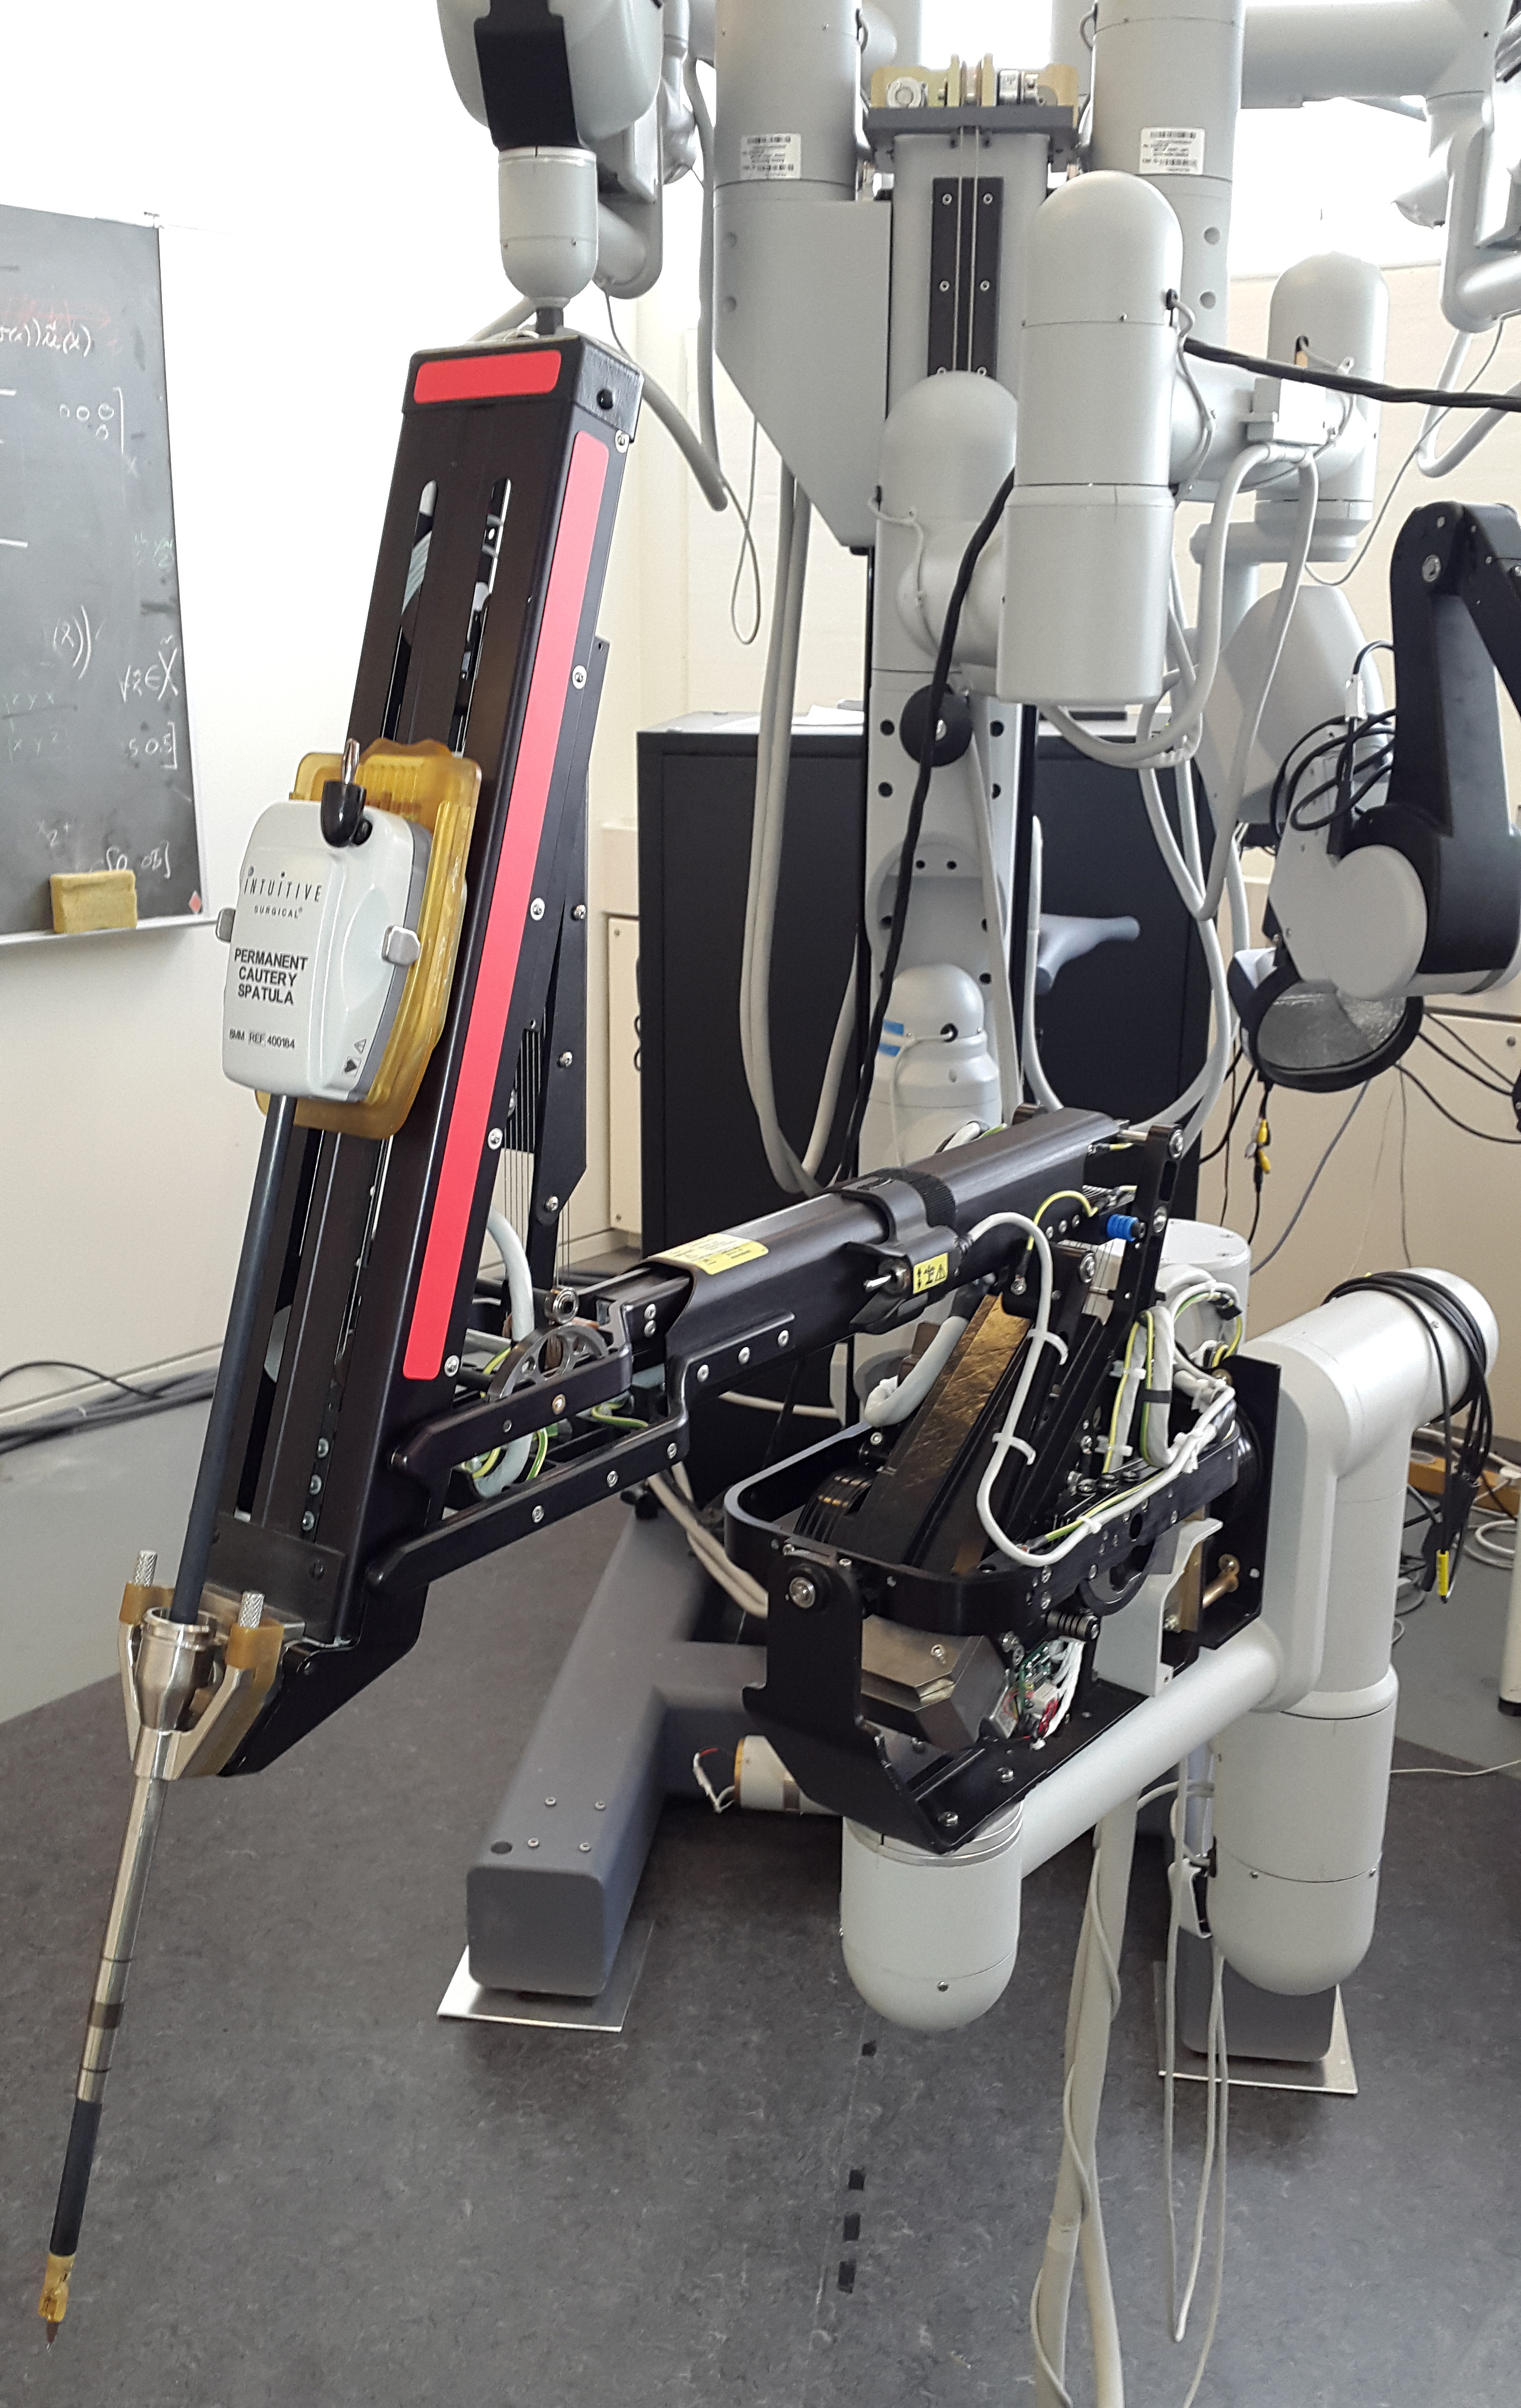
\includegraphics[width=1\textwidth]{20150517_120236.jpg}
%	\end{figure}
%\end{minipage}
%\vspace{1cm}
%\end{frame}

\section{Barrierecertifikater}
\begin{frame}{Barrierecertifikater}{Formelt bevis for garanteret sikkerhed}
\vspace{2mm}
\begin{block}{Definition af sikkerhed}
	\begin{itemize}
		\item Systemets tilstande er i $\mathcal{X}$
		\item Usikre tilstande er i $\mathcal{X}_u\subset\mathcal{X}$ og sikre tilstande i $\mathcal{X}_0\subseteq\mathcal{X}\setminus\mathcal{X}_u$
		\item Nulniveaukurven af $B(\textbf{x})$ danner  barriere mellem $\mathcal{X}_0$ og $\mathcal{X}_u$
	\end{itemize}
\end{block}
\begin{figure}[h]
	\centering
	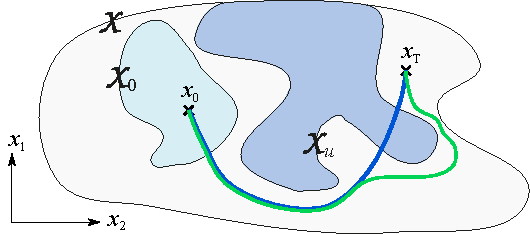
\includegraphics[width=0.8\textwidth]{safety.pdf}
\end{figure}
\vspace{1cm}
\end{frame}

\section{Kontroldesign}
\begin{frame}{Kontrolbarrierefunktioner (CBF)}{Konstruktion af CBF til design af sikkerhedsregulator}
	\vspace{2mm}
\begin{block}{To regulatorer}
	\begin{itemize}
		\item Lineær positionskontrol indenfor det sikre område $\mathcal{X}_0$
		\item Gradvis overgang til sikkerhedsregulator nær $\mathcal{X}_u$
		\item Designet vha. CLF så krav til sikkerhed bliver opfyldt
	\end{itemize}
\end{block}
\vspace{-2mm}
\begin{equation*}
u(\mathbf{x},\tilde{u})=\sigma(\mathbf{x})k_0(\mathbf{x})+(1-\sigma(\mathbf{x}))\tilde{u}(\mathbf{x})
\end{equation*}

\begin{figure}[h]
	\centering
	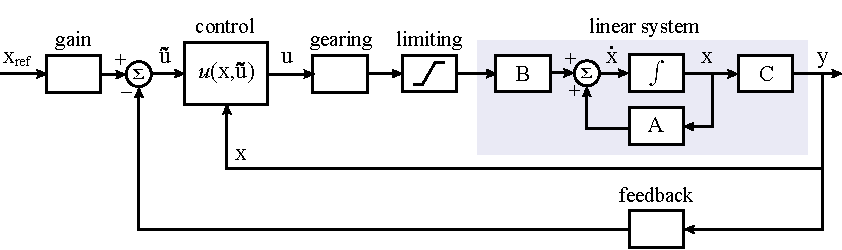
\includegraphics[width=0.9\textwidth]{control_system.pdf}
\end{figure}
	\vspace{5mm}
\end{frame}

{\aauwavesbg%
\begin{frame}[plain,noframenumbering]%
  \finalpage{Demo}
\end{frame}}
%%%%%%%%%%%%%%%%

\end{document}
